\subsection{Transfer: the guarantee does not survive a new batch unless it is recalibrated}\label{sec:res-transfer}

With a whole battery batch held out, calibration and test units are no longer exchangeable, and the guarantee failed as the protocol predicted (H5a). Calibrated on the other two batches, CNA at $\alpha=0.10$ failed on 0\,\% of batch~1 but on 74\,\% of batch~2 and 61\,\% of batch~3 (Table~\ref{tab:transfer}, Fig.~\ref{fig:transfer}). The shortest-lived batch was the worst, the direction expected when a regressor trained mostly on longer-lived cells overestimates remaining life. CNA-DA failed on 45\,\% and 36\,\%, and in the worst cost cell it cost 24 times as much as the cheapest policy. The same loss of validity appeared on N-CMAPSS with a flight-data subset held out: 29--40\,\% failures on three of nine subsets and 0--2\,\% on the other six. Conservative uncertified rules did better under this shift: the one-standard-error cost-tuned alarm failed on 0--2\,\% of the held-out battery cells and the capacity-trend policies on none. Their extra margin, which cost them little within batches, protected them across batches; a calibrated alarm has, by design, no margin beyond what its calibration units require.

Recalibration with pilot units of the new batch restored the guarantee (H5b). Using 10 randomly chosen cells of the held-out batch as calibration units and testing on the rest, the mean failure rate over 300 draws was 7.5--10.1\,\% at $\alpha=0.10$ across batches, lead times and repetitions (8.4--9.5\,\% at the primary lead time), around the exact value $1/11=9.1\,\%$ of Proposition~\ref{prop:cost}; with 20 pilot cells it was 8.3--10.4\,\%. Mean notice at a planned replacement was 48--60 cycles with 10 pilot cells, against 37 cycles on batches 2 and 3 under cross-batch calibration, where most cells failed. Five pilot cells cannot certify $\alpha=0.10$ ($1/(m+1)>\alpha$) and certify $\alpha=0.20$ with a failure rate of 16.5--16.7\,\%. The capacity-trend signal behaved the same way: calibrated across batches it failed on 56\,\% of batch~2, and with 10 pilot cells on 9\,\%. Because pilot cells need not run to failure (Theorem~\ref{thm:cens}), a new batch can be calibrated from the first cells replaced under a conservative interim level; Section~\ref{sec:res-cens} shows that censoring of this kind costs little.

\begin{table*}[t]\footnotesize\setlength{\tabcolsep}{4.5pt}
\caption{Failure before replacement with a whole group held out (battery: lead time 30 cycles; N-CMAPSS: 10 cycles), mean of three repetitions. Pilot: CNA calibrated on $m$ randomly chosen units of the held-out group and tested on the rest (mean over 300 draws); with $m=5$, $\alpha=0.10$ is not attainable and $\alpha=0.20$ is shown.}\label{tab:transfer}
\resizebox{\textwidth}{!}{%
\begin{tabular}{@{}lllllllll@{}}
\toprule
Held-out group (units) & CNA 0.10, other groups & CNA-DA & Pilot $m=10$, $\alpha=0.10$ & Pilot $m=5$, $\alpha=0.20$ & STW window & STW 1-SE & Kamariotis P1 opt. & Trend 1-SE \\
\midrule
Battery batch 1 (36) & 0.00 & 0.00 & 0.095 & 0.167 & 0.00 & 0.00 & 0.00 & 0.00 \\
Battery batch 2 (43) & 0.74 & 0.45 & 0.094 & 0.165 & 0.35 & 0.00 & 0.12 & 0.00 \\
Battery batch 3 (44) & 0.61 & 0.36 & 0.084 & 0.167 & 0.06 & 0.02 & 0.17 & 0.00 \\
N-CMAPSS, 6 subsets (9--15 each) & 0.00--0.02 & 0.00 & -- & 0.165--0.177 & 0.00--0.02 & 0.00 & 0.00 & -- \\
N-CMAPSS subset 4 (10) & 0.33 & 0.10 & -- & 0.165 & 0.07 & 0.10 & 0.07 & -- \\
N-CMAPSS subset 8 (15) & 0.29 & 0.18 & -- & 0.169 & 0.11 & 0.18 & 0.11 & -- \\
N-CMAPSS subset 9 (10) & 0.40 & 0.07 & -- & 0.169 & 0.10 & 0.13 & 0.03 & -- \\
\bottomrule
\end{tabular}}
\end{table*}

\begin{figure*}[t]\centering
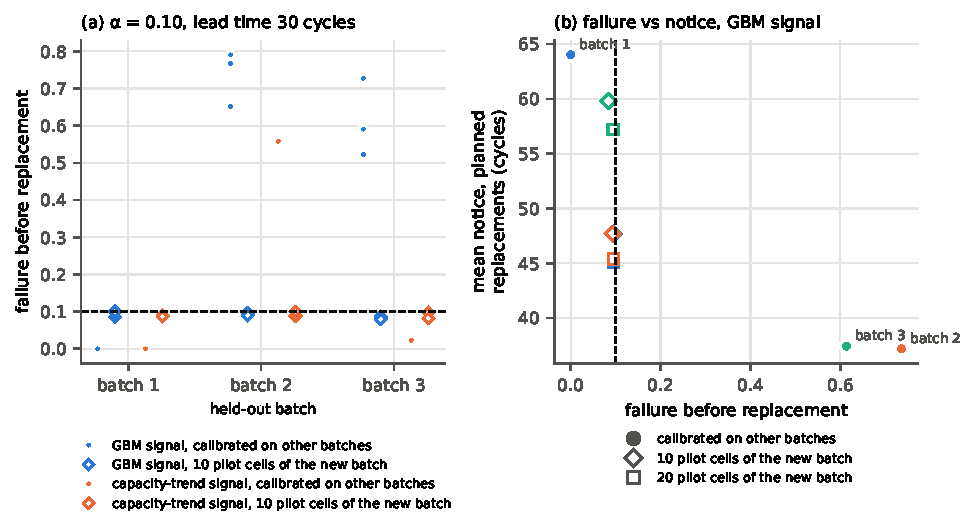
\includegraphics[width=0.85\textwidth]{figures/Fig5_transfer.pdf}
\caption{Battery cells with a whole batch held out ($\alpha=0.10$, lead time 30 cycles). (a) Failure before replacement when the alarm is calibrated on the other batches (dots: three repetitions) or on 10 pilot cells of the held-out batch (diamonds: mean over 300 random draws). (b) Failure against mean notice at planned replacements for the gradient-boosted signal.}\label{fig:transfer}
\end{figure*}

\subsection{What the window score measured}\label{sec:res-window}

Proposition~\ref{prop:window} says that the window scores of the estimate and of a constant can differ only through units whose notice falls near an edge of the constant's acceptance band. On every dataset the reported estimate was pinned below the level as part~(iii) states (100\,\% of alarms within $[H-k\delta^+,H]$) and varied much less than the notice: its standard deviation was 2.3--3.2 cycles on the engines against 4.9--18.0 for the notice (battery 6.3 against 12.9). Discordant units, correct under one report and not the other, were 6.9--14.0\,\% on PHM08 and C-MAPSS, 11.4\,\% on the battery cells and 30.3\,\% on N-CMAPSS (Table~\ref{tab:window}).

The equivalence test of the protocol was not supported. With a margin of $\pm5$ points, estimate and constant were equivalent only on FD002; on FD001, FD003 and N-CMAPSS the intervals were too wide to decide; on PHM08 and FD004 the constant was significantly \emph{better} than the model's estimate ($-6.4$ and $-6.0$ points), and on the battery cells the estimate was significantly better ($+9.8$ points), the one dataset where the estimate's spread at the alarm was a sizeable fraction of the window width (6.3 of 45 cycles). This corrects the earlier summary that the estimate changed the score by at most 3.6 points~\cite{prior}. The plug-in bound of part~(ii), computed on calibration units, exceeded the realised score difference on 6 of 7 datasets and the realised discordance on 4 of 7; it uses estimated probabilities and is not a guarantee. For this article the conclusion is the one that motivates the method: a window score bounds neither the notice nor the failure probability, so neither should be inferred from it.

\begin{table*}[t]\footnotesize\setlength{\tabcolsep}{4.5pt}
\caption{Window score of the window-tuned alarm's estimate and of one constant at the same alarm times ($H=20$ cycles; battery 60), repetition~0. Difference: estimate $-$ constant with Tango 90\,\% interval; equivalence margin $\pm5$ points. SD at the alarm in cycles. Bound: Proposition~\ref{prop:window}(ii) estimated on calibration units; Disc.: realised share of discordant units.}\label{tab:window}
\resizebox{\textwidth}{!}{%
\begin{tabular}{@{}lllllllll@{}}
\toprule
Dataset & $n$ & Estimate (\%) & Constant (\%) & Discordant (est./const.) & Difference (90\,\% CI) & TOST $p$ & SD estimate / notice & Bound / Disc. (points) \\
\midrule
PHM08 & 218 & 87.6 & 94.0 & 4 / 18 & $-6.4$ ($-10.3$, $-3.1$) & 0.756 & 2.6 / 4.9 & 15.9 / 10.1 \\
FD001 & 100 & 86.0 & 85.0 & 6 / 5 & $+1.0$ ($-4.9$, $+7.0$) & 0.126 & 3.0 / 5.3 & 19.1 / 11.0 \\
FD002 & 260 & 90.4 & 91.9 & 7 / 11 & $-1.5$ ($-4.5$, $+1.2$) & 0.028 & 2.4 / 5.2 & 13.6 / 6.9 \\
FD003 & 100 & 84.0 & 86.0 & 6 / 8 & $-2.0$ ($-8.6$, $+4.5$) & 0.216 & 2.9 / 5.3 & 13.6 / 14.0 \\
FD004 & 249 & 79.1 & 85.1 & 6 / 21 & $-6.0$ ($-9.7$, $-2.7$) & 0.694 & 2.3 / 18.0 & 15.2 / 10.8 \\
N-CMAPSS & 99 & 52.5 & 56.6 & 13 / 17 & $-4.0$ ($-13.3$, $+5.2$) & 0.431 & 3.2 / 11.0 & 28.1 / 30.3 \\
Battery & 123 & 95.1 & 85.4 & 13 / 1 & $+9.8$ ($+5.4$, $+15.3$) & 0.964 & 6.3 / 12.9 & 8.9 / 11.4 \\
\bottomrule
\end{tabular}}
\end{table*}
